\chapter{Program do sterowania pomiarami charakterystyk laserów półprzewodnikowych z wykorzystaniem sprzętu Thorlabs}
\section{Wstęp}
W ramach pracy inżynierskiej zostały stworzone programy do sterowania pomiarami charakterystyk laserów.
Program został napiany w dwóch wersjach: skryptowej oraz okienkowej. Podstawą działania programów są następujące klasy:
\begin{itemize}
\item $\mathtt{device.py}$ --- główna klasa, zawiera funkcje: do sprawdzania dostępnych urządzeń,
zwraca instancje danego urządzenia, co umażliwa korzystanie z jego funkcji.
\item $\mathtt{IODevice.py}$ --- klasa do operacji wejścia-wyjścia na programowalnych urządzeniach pomiarowych.
\item $\mathtt{LDC4005.py}$ --- klasa zawierająca funkcje od obsługi zasilacza diód laserowych Thorlabs 4005.
\item $\mathtt{PM100.py}$ --- klasa zawierająca funkcje do obsługi detektora mocy Thorlabs PM100.
\end{itemize}
\section{Wersja skryptowa programu}
Jedna z możliwością przeprowadzania pomiarów jest wykorzystanie skryptu (wraz z innymi klasami dołączony jest do pracy).
Struktura programu pokazana jest na rysunku \ref{struktura_rys_1}. Aby zainstalować wszystkie niezbedne biblioteki należy
w konsoli wywołać polecenie $\mathtt{make}$.
\begin{lstlisting}[style=Bash]
student@ubuntu:~$ make
\end{lstlisting}
Nastepnie uruchamiamy wirtualne środowisko (linia 1), które posiada wszystkie potrzebne biblioteki, następnie
przechodzimy do katologu $\mathtt{examples}$, gdzie znajduje się plik $\mathtt{measure.py}$, który należy użyć do
przeprowadzenia pomiarów:
\begin{lstlisting}[style=Bash]
student@ubuntu:~$ source venvenv/bin/activate
student@ubuntu:~$ cd examples/
\end{lstlisting}
Do przeprawadzenia pomiarów wywolujemy skrypt $\mathtt{measure.py}$ z parametrami:
\begin{itemize}
\item nr: liczba punktów do pomiaru
\item sc: początkowa wartość prądu w mA, od którego należy rozpocząć pomiar
\item ec: wartość prądu w mA do którego przeprowadza się pomiar.
\item fn: nazwa wynikowa pliku z danymi, która będzie zapisana w katalogu $\mathtt{output}$
\end{itemize}
\begin{lstlisting}[style=Bash]
student@ubuntu:~$ python3 measure.py -nr 150 -sc 0 -ec 20
-fn dane
\end{lstlisting}
\begin{figure}
\center
  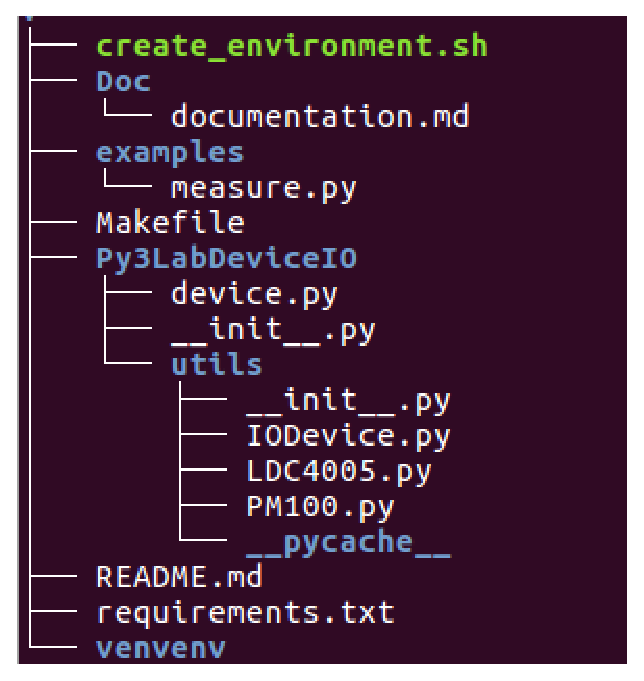
\includegraphics[scale=0.3]{tree.eps}
  \caption{Teoria.}
  \label{struktura_rys_1}
\end{figure}
\section{Wersja okienkowa programu do pomiarów}
Na rysunku \ref{gui_rys} przedstawiony jest okienkowy program do wykonywania charakterystyk. Program napisany jest w języku
Python z wykorzystaniem bibliotek PyQt5, matplotlib
\begin{figure}[h]
\center
  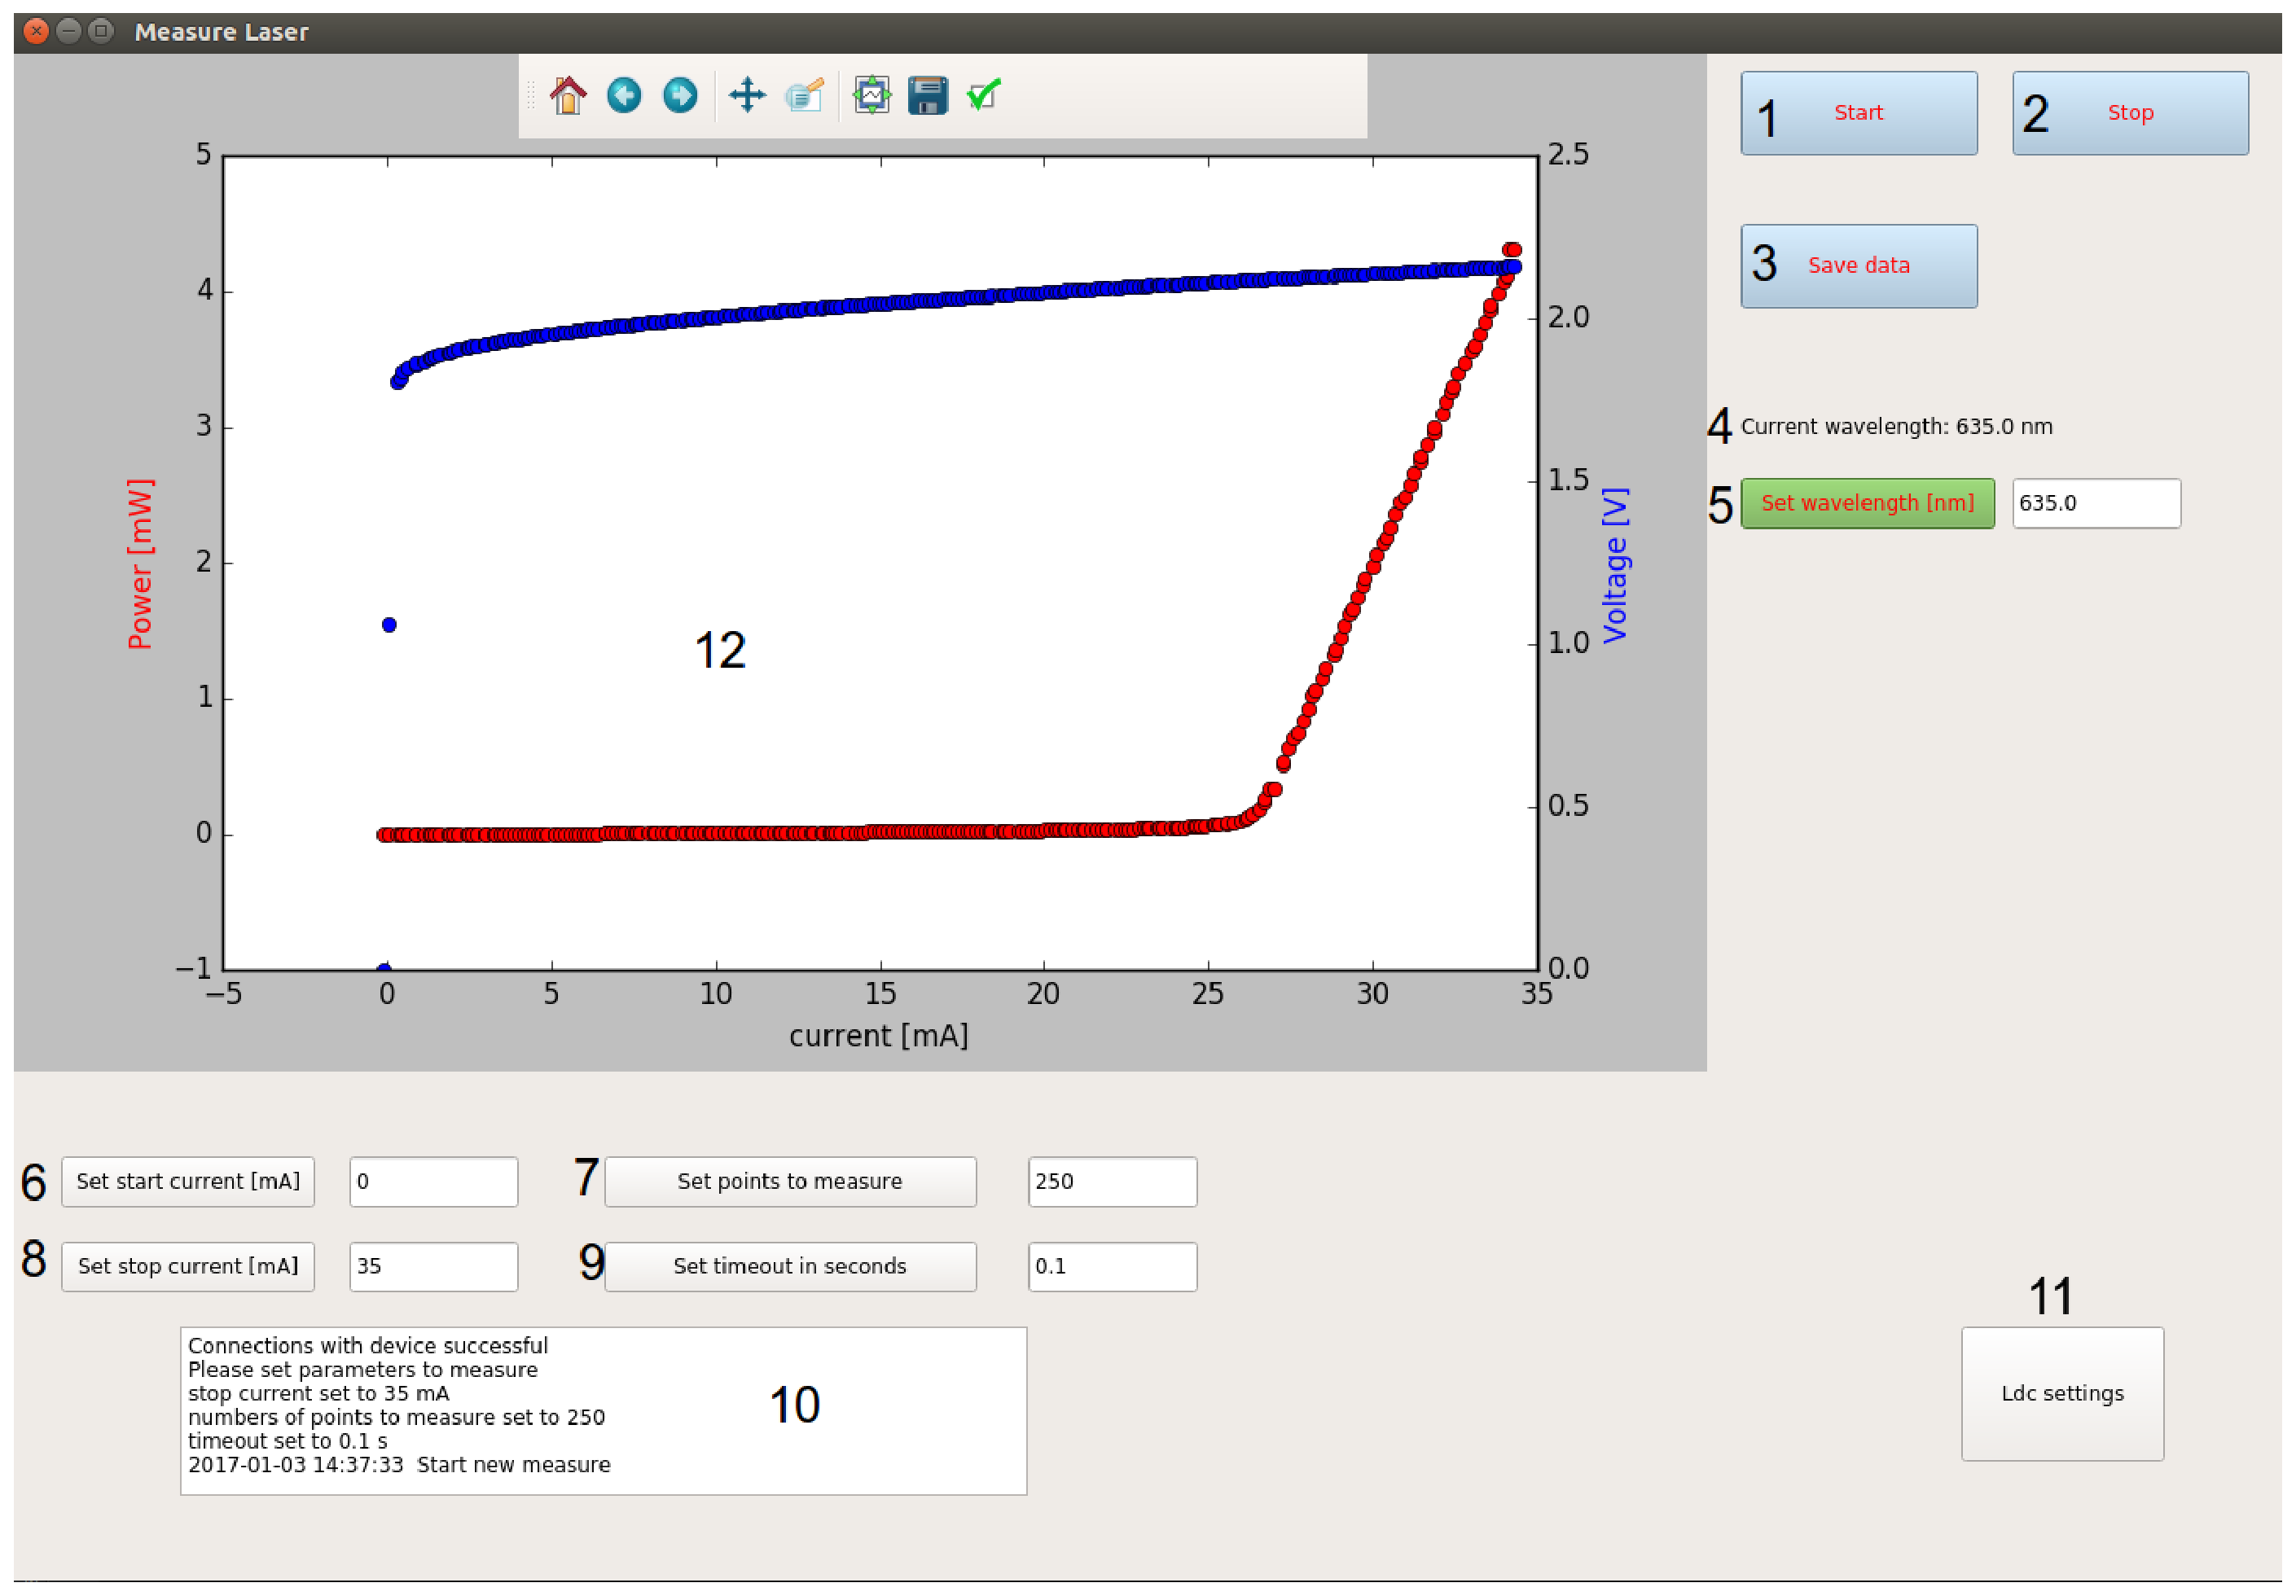
\includegraphics[scale=0.35]{gui.eps}
  \label{gui_rys}
  \caption{1 --- rozpoczecie pomiarów, 2 --- zatrzymanie pomiarów, 3 --- zapisanie danych pomiarowych, 4 --- pokazuje długość fali detektora, 5 --- zmiana długości fali detektora 6 --- ustawia prąd początkowy do pomiarów, 7 ---.}
\end{figure}
\begin{itemize}
\item Przycisk ,,Start" [1] służący do rozpoczęcia pomiarów. Po jego wciśnięciu nastąpi wykonanie charakterystyki lasera na podstawie ustawionych parametrów.
\item Przycisk ,,Stop" [2] służący do zatrzymania pomiarów. Po jego wciśnięciu nastąpi wyłączenie zasilacza.
\item Przycisk ,,Save data" [3] służący do zapisania zebranych danych. Po wciśnięciu należy wybrać ścieżkę. Zapis dokonywany jest w formacie txt.
\item Wyświetlacz długości fali wybranej na detektorze [4]. Długość fali wyświetlana jest w nanometrach.
\item Przycisk służący do zmiany długości fali na detektorze [5]. Wartość należy wprowadzić w nanometrach i zatwierdzić.
\item Przycisk ,,Set start current" [6] --- służy do wybrania prądu, od jakiego ma się zacząć pomiar w mA.
\item Przycisk ,,Set points to measure" [7] --- służy do wybrania ilości punktów do charakterystyki.
\item Przycisk ,,Set stop current" [8] --- służy do wybrania granicy prądu, do jakiego ma się odbyć pomiar w mA.
\item Przycisk ,,Set timeout in seconds" [9] --- służy do ustawienie długości pauzy między zadaniem prądu do zasilacza, a wykonaniem pomiaru.
\item Okienko informacyjne [10] --- wyświetla informacje o pomiarze.
\item Przycisk "Ldc settings" [11] --- ustawia najważniejsze parametry zasilacza diod takie jako wartość maksymalna prądu.
\end{itemize}